\documentclass[UTF8]{article}
% 中文支持
\usepackage[UTF8]{ctex}	
% pdf调用 封面
\usepackage{pdfpages}
% color宏包
\usepackage{color}  
% 导入图片
\usepackage{caption}
\usepackage{graphicx, subfig}
% 防止图片乱跑
\usepackage{float}
% 支持数学符号
\usepackage{amsmath}
% 支持代码块
\usepackage{listings}
% pdf加入大纲
\usepackage{hyperref}
% 去红框
\hypersetup{hidelinks,
	colorlinks=true,
	allcolors=black,
	pdfstartview=Fit,
	breaklinks=true
}


% 设置页面的环境,a4纸张大小,左右上下边距信息
\usepackage[a4paper, left=31.8mm, right=31.8mm, top=25.4mm, bottom=25.4mm]{geometry}

% 代码块的基本设置
\lstset{
 columns=fixed,       
 numbers=left,                                        % 在左侧显示行号
 numberstyle=\tiny\color{gray},                       % 设定行号格式
 frame=none,                                          % 不显示背景边框
 backgroundcolor=\color[RGB]{245,245,244},            % 设定背景颜色
 keywordstyle=\color[RGB]{40,40,255},                 % 设定关键字颜色
 numberstyle=\footnotesize\color{darkgray},           
 commentstyle=\it\color[RGB]{0,96,96},                % 设置代码注释的格式
 stringstyle=\rmfamily\slshape\color[RGB]{128,0,0},   % 设置字符串格式
 showstringspaces=false,                              % 不显示字符串中的空格
 language=matlab,                                        % 设置语言
}

\begin{document}

\begin{titlepage}
% 封面信息

\includepdf[pages={1}]{cover.pdf}
\end{titlepage}

% 生成目录
\tableofcontents
\cleardoublepage

%
\section{实验简介}
%%
\subsection{实验目标}

% 无序列表
\begin{enumerate}
    \item 加深对线性系统分析与设计理论知识的理解与掌握;
    \item 掌握基于MATLAB软件的系统建模/分析/设计/常用方法。
\end{enumerate}

%%
\subsection{实验内容}

\begin{itemize}
    \item 《线性系统分析与设计》理论知识。系统分析/设计/仿真一些方法;
    \item 三大部分:系统模型部分、系统分析部分、系统设计部分;
    \item 参考资料:讲义PPT,相关参考教材。
\end{itemize}


%%
\subsection{实验平台}

MATLAB数学仿真软件


% 第二章
\section{系统模型部分实验}
%%
\subsection{实验目标}

\begin{enumerate}
    \item 掌握不同模型的MATLAB描述方法;
    \item 掌握利用MATLAB进行传递函数模型和状态空间模型相互转换;
    \item 掌握利用MATLAB求解系统的线性变换。
\end{enumerate}

%%
\subsection{实验内容1}
%%%
\subsubsection{实验要求}

\begin{itemize}
    \item 利用MATLAB获取如下系统的传递函数模型、状态空间模型(相关参数可自由取值)。
    \item 利用Simulink搭建上述模型,并观察其单位阶跃响应(相关参数可自由取值)。
\end{itemize}
\begin{figure}[H]
    \centering % 居中 
    % 图片文件的相对路径
    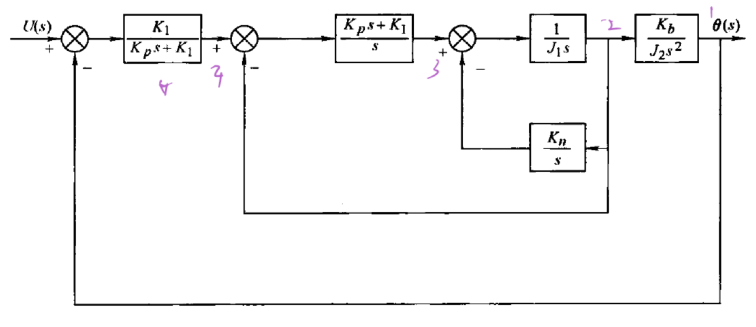
\includegraphics[width=.8\textwidth]{figure/exp1_1.png} 
    \caption{题图} % caption是图片的标题
    % \label{img} % 此处的label相当于一个图片的专属标志,目的是方便上下文的引用
\end{figure}


%%%
\subsubsection{实验程序}
\paragraph{思路}
\begin{enumerate}
    \item 通过系统方块图可以求得系统模拟结构图,获得系统的状态方程,进而获得系统的状态空间表达式如下:
$$
\begin{cases}
    \dot{x} = 
    \begin{bmatrix}
        0 & 1 & 0 & 0 & 0 & 0 \\
        0 & 0 & \frac{K_b}{J_2} & 0 & 0 & 0 \\
        0 & 0 & -\frac{K_p}{J_1} & -\frac{K_n}{J_1} & \frac{1}{J} & \frac{K_p}{J_1} \\
        0 & 0 & 1 & 0 & 0 & 0 \\
        0 & 0 & -K_1 & 0 & 0 & K_1 \\
        -\frac{K_1}{K_p} & 0 & 0 & 0 & 0 & -\frac{K_1}{K_p} \\
    \end{bmatrix}x + 
    \begin{bmatrix}
        0 \\
        0 \\
        0 \\
        0 \\
        0 \\
        \frac{K_1}{K_p}
    \end{bmatrix}u \\
    y = [1 \quad 0 \quad 0 \quad 0 \quad 0 \quad 0]x
\end{cases}
$$
    \item 利用MATLAB转换函数$ss(A, B, C, D),\ ss2tf(A, B, C, D)$即可得到系统的状态空间模型和传递函数模型。
\end{enumerate}

\paragraph{程序}
\begin{lstlisting}
clc, clear
% 参数均取1
J1 = 1;
J2 = 1;
Kp = 1;
Kb = 1;
Kn = 1;
K1 = 1;

A = [0 1 0 0 0 0;
    0 0 Kb/J2 0 0 0;
    0 0 -Kp/J1 -Kn/J1 1/J1 Kp/J1;
    0 0 1 0 0 0;
    0 0 -K1 0 0 K1;
    -K1/Kp 0 0 0 0 -K1/Kp];
B = [0; 0; 0; 0; 0; K1/Kp];
C = [1 0 0 0 0 0];
D = 0;

% 状态空间模型
G1 = ss(A, B, C, D)
% 传递函数模型
[num, den] = ss2tf(A, B, C, D);
G2 = tf(num, den)
\end{lstlisting}

\paragraph{Simulink模型}~{}
\\
利用Simulink搭建上述模型,如下图所示:
\begin{figure}[H]
    \centering % 居中 
    % 图片文件的相对路径
    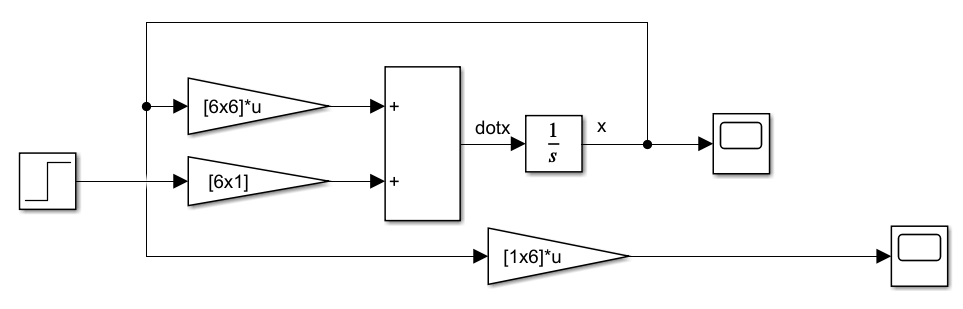
\includegraphics[width=.8\textwidth]{figure/exp1_1_model.png} 
    \caption{Simulink模型} % caption是图片的标题
    % \label{img} % 此处的label相当于一个图片的专属标志,目的是方便上下文的引用
\end{figure}

%%%
\subsubsection{实验结果}
\paragraph{MATLAB运行结果}~{}
\\
状态空间模型:
\begin{align*}
    A &= 
    \begin{bmatrix}
        0 & 1 & 0 & 0 & 0 & 0 \\
        0 & 0 & 1 & 0 & 0 & 0 \\
        0 & 0 & -1 & -1 & 1 & 1 \\
        0 & 0 & 1 & 0 & 0 & 0 \\
        0 & 0 & -1 & 0 & 0 & 1 \\
        -1 & 0 & 0 & 0 & 0 & -1 \\
    \end{bmatrix} \\
    B &= 
    \begin{bmatrix}
        0 \\
        0 \\
        0 \\
        0 \\
        0 \\
        1
    \end{bmatrix} \\
    C &= [1 \quad 0 \quad 0 \quad 0 \quad 0 \quad 0] \\
    D &= 0
\end{align*}
传递函数模型:
$$
    G_2 = \frac{s^2 + s}{s^6 + 2s^5 + 3s^4 + 2s^3 + s^2 + s}
$$
系统的单位阶跃响应:
\begin{figure}[H]
    \centering % 居中 
    % 图片文件的相对路径
    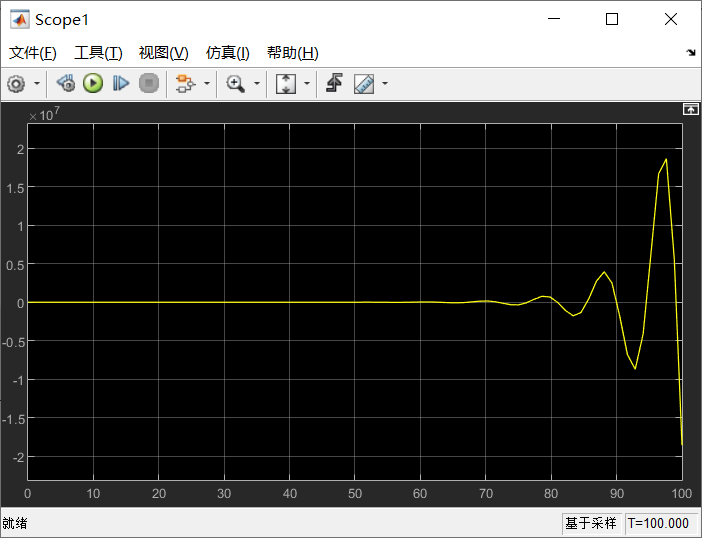
\includegraphics[width=.8\textwidth]{figure/exp1_1_系统单位阶跃响应.png} 
    \caption{系统单位阶跃响应} % caption是图片的标题
    % \label{img} % 此处的label相当于一个图片的专属标志,目的是方便上下文的引用
\end{figure}


%%
\subsection{实验内容2}
%%%
\subsubsection{实验要求}

\begin{itemize}
    \item 利用Simulink搭建如下系统结构框图;
    \item 选初始条件[-0.2; 0.3; 0.7],观察系统的状态响应(用Simulink的示波器模块看)。
\end{itemize}

\begin{figure}[H]
    \centering % 居中 
    % 图片文件的相对路径
    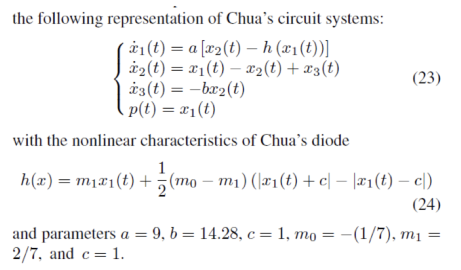
\includegraphics[width=.8\textwidth]{figure/exp1_2.png} 
    \caption{题图} % caption是图片的标题
    % \label{img} % 此处的label相当于一个图片的专属标志,目的是方便上下文的引用
\end{figure}


%%%
\subsubsection{实验程序}
\paragraph{Simulink模型}~{}
\\
利用Simulink搭建上述模型,如下图所示:
\begin{figure}[H]
    \centering % 居中 
    % 图片文件的相对路径
    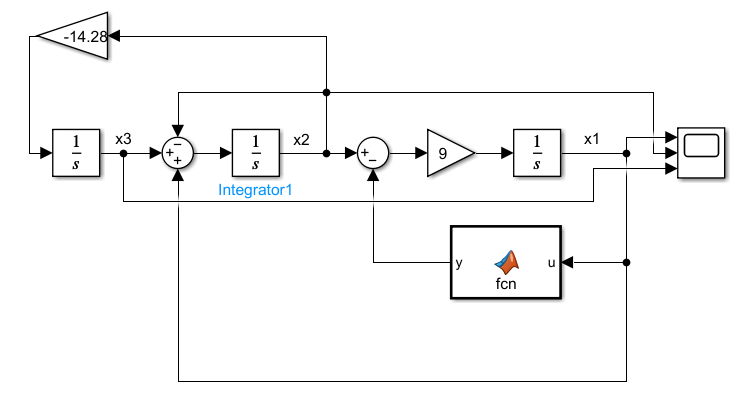
\includegraphics[width=.8\textwidth]{figure/exp1_2_model.png} 
    \caption{Simulink模型} % caption是图片的标题
    % \label{img} % 此处的label相当于一个图片的专属标志,目的是方便上下文的引用
\end{figure}
\noindent 其中函数$fcn$代码如下:
\begin{lstlisting}
function y = fcn(u)
%m0 = -(1/7);
%m1 =  2/7;
%c = 1;
%y = m1 * u + (m0-m1)/2*(abs(u + c)-abs(u - c));
y = 2/7 * u + (-(1/7)-2/7)/2*(abs(u + 1)-abs(u - 1));
\end{lstlisting}


%%%
\subsubsection{实验结果}
\paragraph{MATLAB运行结果}~{}

选取初始条件分别为$[-0.2; 0.3; 0.7]$,运行上述Simulink模型后得到系统的状态响应如下图所示:
\begin{figure}[H]
    \centering % 居中 
    % 图片文件的相对路径
    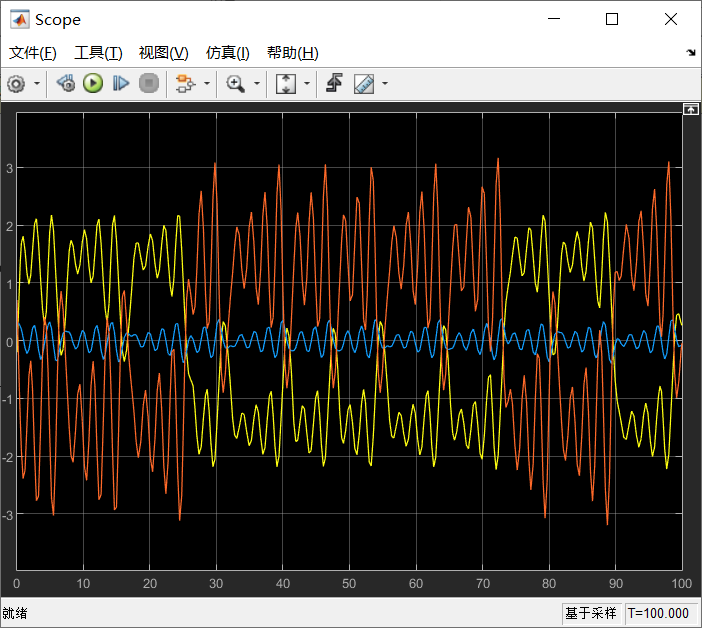
\includegraphics[width=.8\textwidth]{figure/exp1_2_系统的状态响应.png} 
    \caption{系统的状态响应} % caption是图片的标题
    % \label{img} % 此处的label相当于一个图片的专属标志,目的是方便上下文的引用
\end{figure}

%%
\subsection{小结}
在进行第一个实验内容时,首先尝试了如下方法:将模型分解为五个子模型,并利用MATLAB内置函数$tf(num, den)$得到它们的传递函数模型;然后利用$feedback()$函数构成反馈,得到整体系统的传递函数模型;最后利用转换函数$tf2ss()$将系统的传递函数模型转换为状态空间模型。但是,利用此方法得到的模型结果始终存在错误,在多次检查未发现问题的情况下决定直接根据系统方块图得到系统模拟结构图,以获取系统的状态空间模型方程和传递函数模型。

利用Simulink中的示波器模块查看系统响应时,应注意合理调节窗口显示图像的时间长度,此处调整为100s为宜。


% 第三章
\section{系统分析部分实验}
%%
\subsection{实验目标}

\begin{enumerate}
    \item 学习利用MATLAB求解线性定常系统的状态转移矩阵;
    \item 学习利用MATLAB判断控制系统的能观性与能控性;
    \item 掌握利用MATLAB求解系统的解、判断系统能控性与能观性的方法;
    \item 熟练掌握李雅普诺夫稳定性概念及其判别方法;
    \item 掌握使用MATLAB求解特征值判别系统稳定性的方法;
    \item 掌握使用MATLAB计算李雅普诺夫方程的解来判别系统稳定性的方法。
\end{enumerate}

%%
\subsection{实验内容1}
%%%
\subsubsection{实验要求}
判断如下系统的稳定性:
\begin{figure}[H]
    \centering % 居中 
    % 图片文件的相对路径
    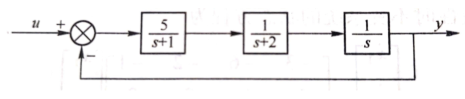
\includegraphics[width=.8\textwidth]{figure/exp2_1.png} 
    \caption{题图} % caption是图片的标题
    % \label{img} % 此处的label相当于一个图片的专属标志,目的是方便上下文的引用
\end{figure}

%%%
\subsubsection{实验程序}
\paragraph{思路}~{}
\\
李雅普诺夫第二法,思路二:
\begin{enumerate}
    \item 选取一个正定矩阵$Q$;
    \item 代入李雅普诺夫方程$A^TP + PA = -Q$,解出矩阵$P$;
    \item 按希尔维斯特判据判定$P$的正定性;
    \item 做出系统是否渐进稳定的结论。
\end{enumerate}
其他方法:通过结构图求出系统的状态空间表达式,进而直接解出系统极点,通过系统矩阵$A$的特征根是否全部具有负实部判断系统的稳定性。

\paragraph{程序}
\begin{lstlisting}
clc
clear
% 通过结构图求状态空间表达式
% dotx_3 = x_2 
% dotx_2 = x_1 - 2 * x_2
% dotx_1 = -x_1 - 5 * x_3 + 5 * u
% y = x_3
% 传递函数中无零点的实现
% A = [0 1 0; 0 0 1; -5 - 2 -3];
% B = [0 0 1]';
% C = [5 0 0];

% 直接法判断稳定性
A = [-1 0 -5; 1 -2 0; 0 1 0];
eig(A)

% 李二法 思路二判断稳定性
Q = eye(size(A, 1));
% 求李雅普诺夫方程
P = lyap(A, Q);

% 利用希尔维斯特判据判断P的正定性
det1 = det(P(1, 1));
det2 = det(P(1 : 2, 1 : 2));
det3 = det(P(1 : 3, 1 : 3));
det4 = det(P);
Det = [det1; det2; det3; det4];
if min(Det) > 0
    '系统稳定'
else
    '系统不稳定'
end
\end{lstlisting}

%%%
\subsubsection{实验结果}
系统稳定,且系统矩阵$A$的特征根为:
\begin{align*}
    -2.9042 + 0.0000i \\
    -0.0479 + 1.3112i \\
    -0.0479 - 1.3112i    
\end{align*}


%%
\subsection{实验内容2}
%%%
\subsubsection{实验要求}

判断如下系统的能控能观性,若不完全能控且不完全能观,求其能控能观子系统:
\begin{figure}[H]
    \centering % 居中 
    % 图片文件的相对路径
    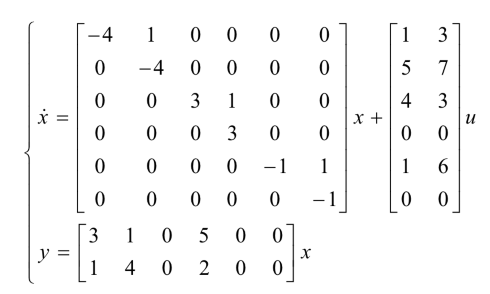
\includegraphics[width=.6\textwidth]{figure/exp2_2.png} 
    \caption{题图} % caption是图片的标题
    % \label{img} % 此处的label相当于一个图片的专属标志,目的是方便上下文的引用
\end{figure}


%%%
\subsubsection{实验程序}
\paragraph{思路}
\begin{enumerate}
    \item 判断系统的能控性;
    \item 系统按能控性分解;
    \item 判断能控子系统的能观性;
    \item 能控子系统按能观性分解;
    \item 得到能控能观子系统。
\end{enumerate}

\paragraph{程序}
\begin{lstlisting}
clc
clear all
A = [-4 1 0 0 0 0; 
    0 -4 0 0 0 0;
    0 0 3 1 0 0;
    0 0 0 3 0 0;
    0 0 0 0 -1 1;
    0 0 0 0 0 -1]
B = [1 3; 5 7; 4 3; 0 0; 1 6; 0 0]
C = [3 1 0 5 0 0; 1 4 0 2 0 0]

n = size(A, 1);
% 能控性矩阵
Qc = ctrb(A, B);
if rank(Qc) == n
    '系统能控'
else
    '系统不完全能控'
    [A1, B1, C1, T, k] = ctrbf(A, B, C)
end

% 能控子系统
% dotx_c = Ac * x_c + Axuc * x_uc + Bc * u
Ac = A1(3 : 6, 3 : 6)
Axuc = A1(3 : 6, 1 : 2)
Bc = B1(3 : 6, :)
Cc = C1(:, 3 : 6)

% 能控子系统判断能观性
% 能观性矩阵
Qo = obsv(Ac, Cc);
if rank(Qo) == n
    '系统能观'
else
    '系统不完全能观'
    [A2, B2, C2, T, k] = obsvf(Ac, Bc, Cc)
end

% 能控子系统按能观性分解,得能控能观子系统
% dotx_ = A2 * x_ + T * Axuc * x_uc + B2 * u
Aco = A2(3 : 4, 3 : 4)
Bco = B2(3 : 4, :)
Cco = C2(:, 3 : 4)
% % = 0
% Axuc = T * Axuc
% Axuc = Axuc(3 : 4, :)
\end{lstlisting}

%%%
\subsubsection{实验结果}
\paragraph{matlab运行结果}~{}
\\
系统不完全能控且不完全能观,其能控子系统为:
\begin{align*}
    Ac &=    
    \begin{bmatrix}
        -3.3080 & -1.6602 & -0.3915 & 0.3681 \\
        -1.0761 & -0.8482 & -2.2992 & -2.4450 \\
        -0.1821 & -2.3817 & 0.1595 & 0.4902 \\
        1.0215 & -2.0818 & 0.7127 & -2.0033        
    \end{bmatrix} \\
    Axuc &= 
    \begin{bmatrix}
        -0.4034 & -0.1596 \\
        0.2830 & 0.6634 \\
        0.7228 & -0.6144 \\
        -0.4845 & -0.3961
    \end{bmatrix} \\
    Bc &= 
    \begin{bmatrix}
        0 & 0 \\
        0 & 0 \\ 
        -2.6403 & 1.5809 \\
        -6.0024 & -10.0250
    \end{bmatrix} \\
    Cc &= 
    \begin{bmatrix}
        2.7299 & 0.1531 & 0.4405 & -1.5266 \\
        1.0135 & -2.2964 & -0.6800 & -3.1995
    \end{bmatrix}
\end{align*}
能控能观子系统为:
\begin{align*}
    Aco &= 
    \begin{bmatrix} 
        -4.4472 & 0.7236 \\
        -0.2764 & -3.5528
    \end{bmatrix} \\
    Bco &= 
    \begin{bmatrix} 
        -1.7780 & -1.1282 \\
        4.7790 & 7.5317
    \end{bmatrix} \\
    Cco &= 
    \begin{bmatrix} 
        2.0262 & 2.4278 \\
        -1.2523 & 3.9283     
    \end{bmatrix} 
\end{align*}

%%
\subsection{小结}
在进行系统的能控性和能观性分解时,发现先进行能控性分解再进行能观性分解,与先进行能观性分解再进行能控性分解,两种不同顺序的方法得到的结果不一致,后来与助教讨论发现该现象是正常情况。这种结果不一致的情况出现的原因在于同一个系统可以有多个不同形式的状态空间表达式。

% 第四章
\section{系统设计部分实验}
%%
\subsection{实验目标}

\begin{enumerate}
    \item 掌握MATLAB控制系统工具箱为极点配置、状态观测器、系统解耦等系统综合提供的专用函数;
    \item 掌握极点配置、全维状态观测器、降维状态观测器的设计方法;
    \item 掌握极点配置与状态观测器相结合的设计方法;
    \item 掌握利用MATLAB设计不同类别控制器的方法。
\end{enumerate}

%%
\subsection{实验内容1}
%%%
\subsubsection{实验要求}

设计状态反馈控制器,使得闭环系统极点为$P1$(自行选择合理数值),验证控制效果:

$$
\begin{cases}
    \dot{x} = 
    \begin{bmatrix}
        -1 & 0 & 0 & 1 \\
        2 & -3 & 0 & 0 \\
        0 & 0 & 2 & 0 \\
        4 & -1 & 2 & -4 \\
    \end{bmatrix} + 
    \begin{bmatrix}
        0 \\
        0 \\
        1 \\
        2 \\
    \end{bmatrix}u \\
    y = [3 \quad 0 \quad 1 \quad 0]x
\end{cases}
$$


%%%
\subsubsection{实验程序}

\paragraph{思路}

\begin{enumerate}
    \item 判断系统的能控性,系统能控则可通过状态反馈任意配置系统极点;
    \item 通过MATLAB内嵌算法函数$acker(),\ place()$,计算系统给定极点下的状态反馈增益。格式:
\begin{align*}
    K = acker(A, b, P) \\
    K = place(A, B, P)
\end{align*}
其中,$P$为目标极点,$K$为反馈增益。注意MATLAB中反馈增益阵$K$与教材上的的差异:
$$
\begin{aligned}
    \text{MATLAB:}& u = -Kx \\
    \text{教材:}& u = Kx
\end{aligned}
$$
\end{enumerate}

\paragraph{程序}
\begin{lstlisting}
clc, clear
A = [-1 0 0 1; 2 -3 0 0; 0 0 2 0; 4 -1 2 -4];
B = [0; 0; 1; 2];
C = [3 0 1 0];
P = [-1, -2, -3, -4];

n = size(A, 1);
% 求能控性矩阵
Qc = ctrb(A, B);
if rank(Qc) == n
    '系统能控'
else
    '系统不完全能控'
end

syms s
% K = -acker(A, B, P)
K = -place(A, B, P)

% 闭环特征方程
f = det(s*eye(4, 4) - (A - B*K))
% 期望特征方程
f_star = (s - P(1))*(s - P(2))*(s - P(3))*(s - P(4))
f_star = taylor(f_star, s)

% 特征根检验
lambda = eig(A + B*K)
\end{lstlisting}

\paragraph{Simulink模型}~{}
\\
原系统和带状态反馈的系统Simulink模型如下图所示:
\begin{figure}[H]
    \centering % 居中 
    % 图片文件的相对路径
    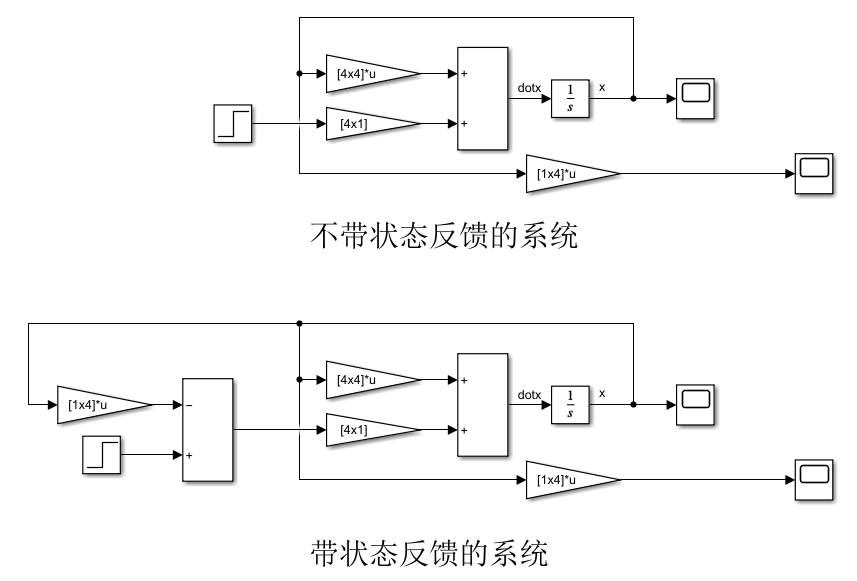
\includegraphics[width=.8\textwidth]{figure/exp3_1_model.png} 
    \caption{题图} % caption是图片的标题
    % \label{img} % 此处的label相当于一个图片的专属标志,目的是方便上下文的引用
\end{figure}


%%%
\subsubsection{实验结果}
原系统完全能控,状态反馈系数矩阵:
$$
K = [-2.04 \quad 0.08 \quad 5.62 \quad -0.81]
$$

\paragraph{单位阶跃激励下的系统输出}~{}
\\
原系统:
\begin{figure}[H]
    \centering % 居中 
    % 图片文件的相对路径
    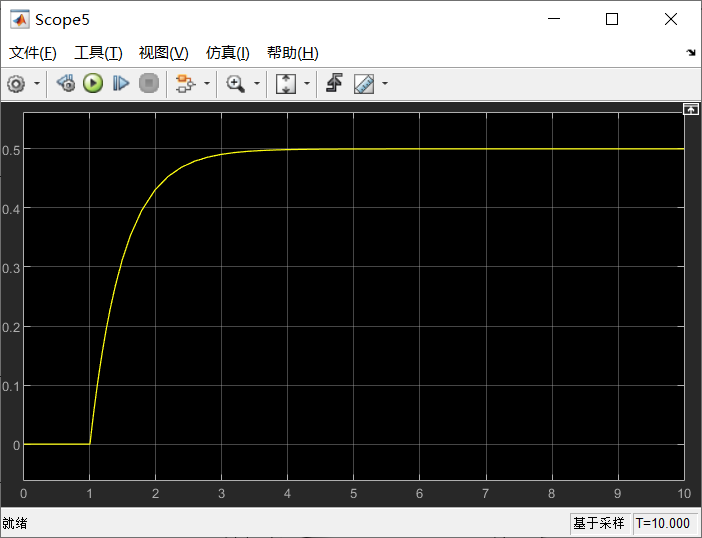
\includegraphics[width=.8\textwidth]{figure/exp3_1_原系统输出.png} 
    \caption{原系统输出} % caption是图片的标题
    % \label{img} % 此处的label相当于一个图片的专属标志,目的是方便上下文的引用
\end{figure}

带状态反馈系统:
\begin{figure}[H]
    \centering % 居中 
    % 图片文件的相对路径
    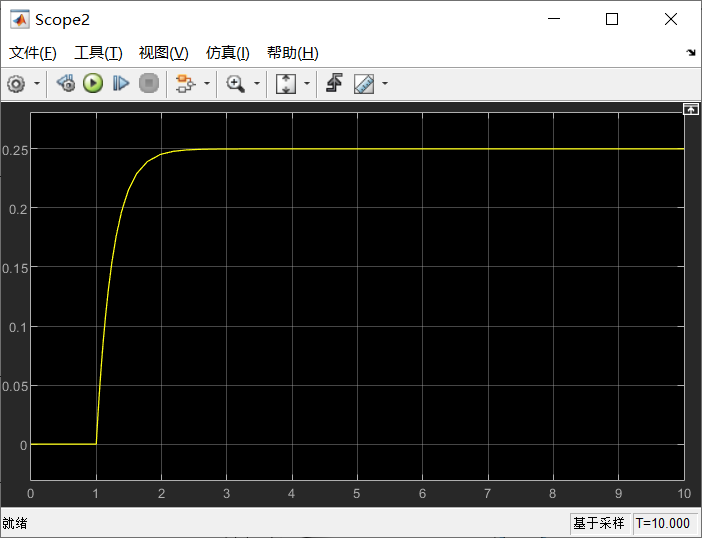
\includegraphics[width=.8\textwidth]{figure/exp3_1_带状态反馈系统输出.png} 
    \caption{带状态反馈系统输出} % caption是图片的标题
    % \label{img} % 此处的label相当于一个图片的专属标志,目的是方便上下文的引用
\end{figure}

\paragraph{系统状态变化}~{}
\\
原系统:
\begin{figure}[H]
    \centering % 居中 
    % 图片文件的相对路径
    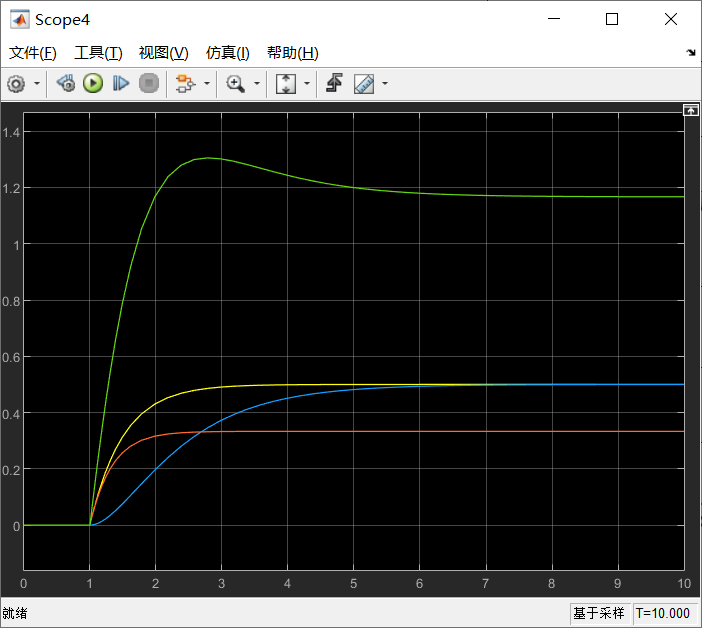
\includegraphics[width=.8\textwidth]{figure/exp3_1_原系统状态.png} 
    \caption{原系统状态变化} % caption是图片的标题
    % \label{img} % 此处的label相当于一个图片的专属标志,目的是方便上下文的引用
\end{figure}

\noindent 带状态反馈系统:
\begin{figure}[H]
    \centering % 居中 
    % 图片文件的相对路径
    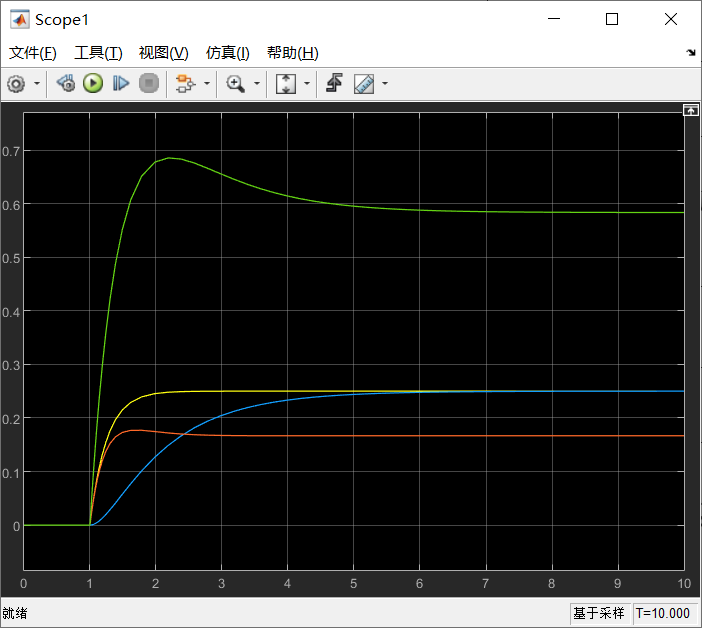
\includegraphics[width=.8\textwidth]{figure/exp3_1_带状态反馈系统状态.png} 
    \caption{带状态反馈系统状态变化} % caption是图片的标题
    % \label{img} % 此处的label相当于一个图片的专属标志,目的是方便上下文的引用
\end{figure}
由以上实验结果分析可知,在单位阶跃激励作用下,带状态反馈系统输出信号的收敛速度明显快于原系统,且状态趋于稳定的时间也更短。

%%
\subsection{实验内容2}
%%%
\subsubsection{实验要求}
设计状态观测器,使得观测误差系统极点为$P2$(自行选择合理数值),验证状态观测效果,系统同上。


%%%
\subsubsection{实验程序}
\paragraph{思路}
\begin{enumerate}
    \item 判断系统的能观性,系统能观则可构造观测器;
    \item 存在如下关系:
$$
\lambda_{(A - GC)} = \lambda_{(A^T - C^TG^T)}
$$
对比$(A^T - C^TG^T),\ (A + BK)$,令$-G^T = K$,则有:
$$
G = acker(A', B', P)'
$$
其中,$P$为给定观测器极点。
\end{enumerate}

\paragraph{程序}
\begin{lstlisting}
clear, clc
A = [-1 0 0 1; 2 -3 0 0; 0 0 2 0; 4 -1 2 -4];
B = [0; 0; 1; 2];
C = [3 0 1 0];
P = [-1, -2, -3, -4];

% 设计状态观测器,极点配置到P
n = 4;
Qo = obsv(A, C);
ro = rank(Qo);
if (ro == n)
    disp('系统是可观测的')
    A1 = A';
    B1 = C';
    G = acker(A1, B1, P)';
    AGC = A - G*C
    % 特征根
    eig(AGC)
elseif (ro ~= n)
    disp('系统是不可观测的,不能进行观测器的设计') 
end
\end{lstlisting}


\paragraph{Simulink模型}~{}
\\
带状态观测器的Simulink模型如下图所示:
\begin{figure}[H]
    \centering % 居中 
    % 图片文件的相对路径
    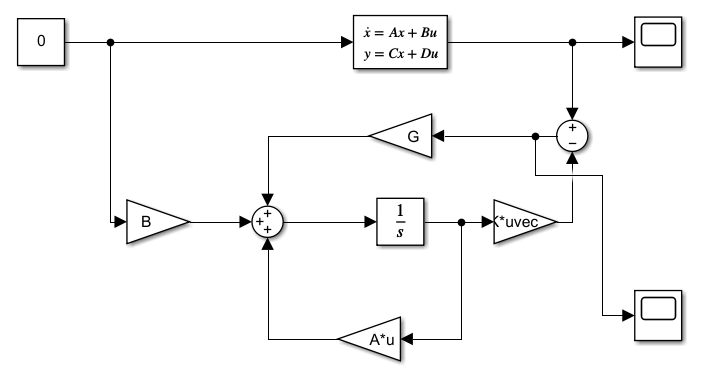
\includegraphics[width=.8\textwidth]{figure/exp3_2_model.png} 
    \caption{带状态观测器的Simulink模型} % caption是图片的标题
    % \label{img} % 此处的label相当于一个图片的专属标志,目的是方便上下文的引用
\end{figure}
其中,原系统的状态初始值设为$[1; 1; 1; 1]$,状态观测器的状态初始值设为$[0; 0; 0; 0]$。


%%%
\subsubsection{实验结果}
\noindent 系统可观测,状态观测器的输出误差反馈矩阵:
$$
G = 
\begin{bmatrix}
0.157 \\
0.196 \\
3.529 \\
1.804 \\
\end{bmatrix}
$$

\noindent 零输入作用下的状态观测误差变化情况:
\begin{figure}[H]
    \centering % 居中 
    % 图片文件的相对路径
    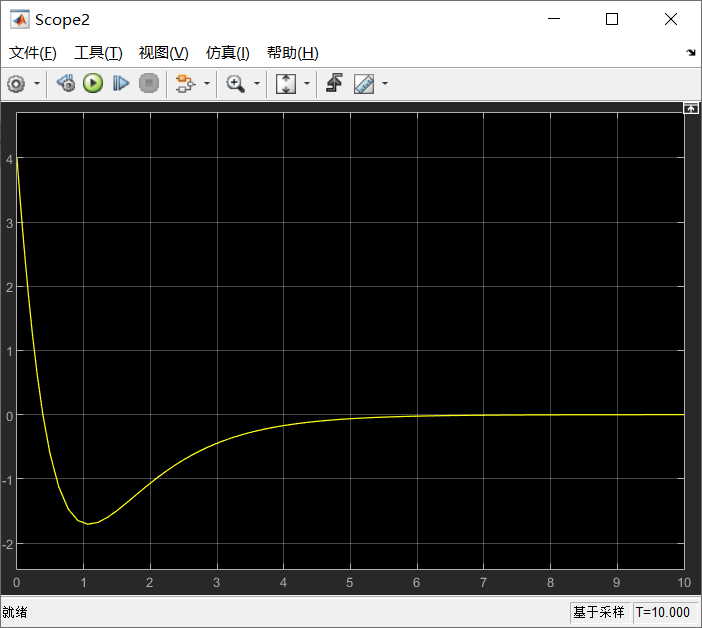
\includegraphics[width=.8\textwidth]{figure/exp3_2_零输入作用下的状态观测误差变化.png} 
    \caption{零输入作用下的状态观测误差变化} % caption是图片的标题
    % \label{img} % 此处的label相当于一个图片的专属标志,目的是方便上下文的引用
\end{figure}
由以上实验结果分析可知,零输入作用下的状态观测误差在短时间内即收敛到0值,说明状态观测值与状态真实值一致,状态观测的效果较好。实验过程中还发现,此状态观测误差的收敛速度还与原系统和状态观测器的初始状态值存在关系。

%%
\subsection{实验内容3}
%%%
\subsubsection{实验要求}
设计基于状态观测器的状态反馈,使得闭环系统极点为$P1$(同第一问数值),验证控制效果,并与基于真实状态反馈控制进行比较,系统同上。

%%%
\subsubsection{实验程序}
\paragraph{思路}
\begin{enumerate}
    \item 判断系统的能观性,系统能观则可任意配置状态观测器极点;
    \item 判断系统的能控性,系统能控则可任意配置闭环系统极点;
    \item 设闭环系统极点为$P1$,状态观测器极点为$P2$,则状态反馈矩阵$K$和状态误差反馈矩阵$G$可由如下命令得到:
\begin{align*}
    K &= acker(A, B, P1) \\
    G &= (acker(A', C', P2))'
\end{align*}
\end{enumerate}

\paragraph{程序}
\begin{lstlisting}
%% 设计基于状态观测器的状态反馈,实现极点配置
clc, clear
A = [-1 0 0 1; 2 -3 0 0; 0 0 2 0; 4 -1 2 -4];
B = [0; 0; 1; 2];
C = [3 0 1 0];
P1 = [-1, -2, -3, -4];
P2 = [-1, -2, -3, -4];

n = size(A);
if rank(obsv(A, C)) == n
    disp('系统能观,可任意配置观测器系统极点')
    G = (acker(A', C', P2))'
else
    disp('系统不完全能观,不可以对观测器系统进行极点任意配置')
end

if rank(ctrb(A, B)) == n
    disp('系统能控,可通过状态反馈任意配置极点')
    K = acker(A, B, P1) % 计算给定极点下的状态反馈增益
else
    disp('系统不完全能控,不可以通过状态反馈实现极点任意配置')
end
\end{lstlisting}

\paragraph{Simulink模型}~{}

基于状态观测器的状态反馈系统和基于真实状态的状态反馈系统的Simulink模型如下图所示:
\begin{figure}[H]
    \centering % 居中 
    % 图片文件的相对路径
    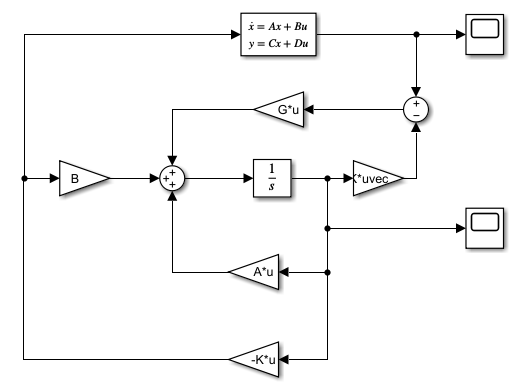
\includegraphics[width=.6\textwidth]{figure/exp3_3_基于状态观测器的状态反馈.png} 
    \caption{基于状态观测器的状态反馈} % caption是图片的标题
    % \label{img} % 此处的label相当于一个图片的专属标志,目的是方便上下文的引用
\end{figure}
\begin{figure}[H]
    \centering % 居中 
    % 图片文件的相对路径
    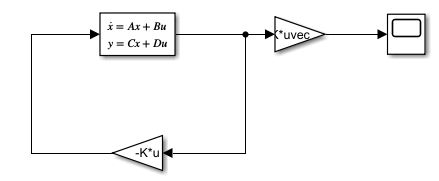
\includegraphics[width=.5\textwidth]{figure/exp3_3_基于真实状态的状态反馈.png} 
    \caption{基于真实状态的状态反馈} % caption是图片的标题
    % \label{img} % 此处的label相当于一个图片的专属标志,目的是方便上下文的引用
\end{figure}
其中,原系统的状态初始值设为$[1; 1; 1; 1]$,状态观测器的状态初始值设为$[0; 0; 0; 0]$。

%%%
\subsubsection{实验结果}
系统能控且能观,指定闭环系统极点$P1$和状态观测器极点$P2$下的状态反馈矩阵$K$和状态误差反馈矩阵$G$分别为:
\begin{align*}
    K &= [-2.038 \quad 0.077 \quad 5.615 \quad -0.808] \\
    G &= 
    \begin{bmatrix}
        0.157 \\
        0.196 \\
        3.529 \\
        1.804
    \end{bmatrix}
\end{align*}

\noindent 基于状态观测器的状态反馈系统输出变化情况:
\begin{figure}[H]
    \centering % 居中 
    % 图片文件的相对路径
    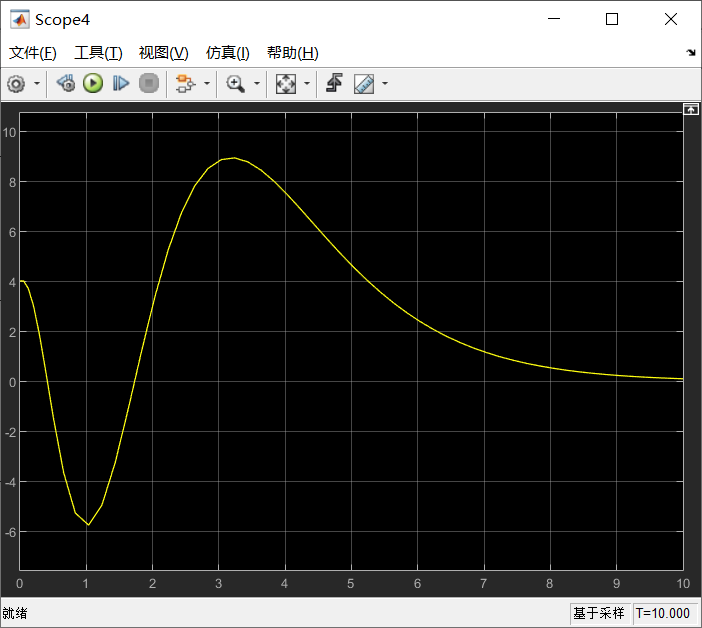
\includegraphics[width=.8\textwidth]{figure/exp3_3_基于状态观测器的状态反馈_输出.png} 
    \caption{基于状态观测器的状态反馈系统输出} % caption是图片的标题
    % \label{img} % 此处的label相当于一个图片的专属标志,目的是方便上下文的引用
\end{figure}

\noindent 基于真实状态的状态反馈系统输出变化情况:
\begin{figure}[H]
    \centering % 居中 
    % 图片文件的相对路径
    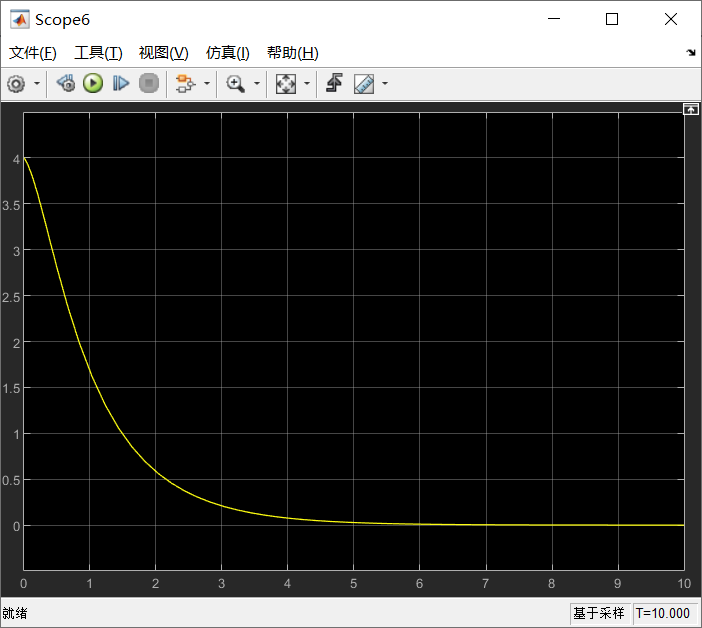
\includegraphics[width=.8\textwidth]{figure/exp3_3_基于真实状态的状态反馈_输出.png} 
    \caption{基于真实状态的状态反馈系统输出} % caption是图片的标题
    % \label{img} % 此处的label相当于一个图片的专属标志,目的是方便上下文的引用
\end{figure}

由以上实验结果分析可知,相比基于状态观测器的状态反馈系统输出,基于真实状态的状态反馈系统输出的收敛速度明显更快,这是由于状态观测器对于状态的观测需要一段时间才能达到比较理想的效果,因而收敛速度相对理想情况下较慢。实验过程中还发现,状态反馈系统的输出变化情况还与系统的状态初始值有关,因此,状态初始值的合理选取也会影响到实验的最终结果。

%%
\subsection{小结}
注意系统镇定与系统极点配置之间的区别:系统镇定只需让系统满足渐进稳定的条件即可,而极点配置则需要将闭环系统的极点配置到指定的位置,以实现给定的性能条件。

基于状态观测器的状态反馈系统相比基于真实状态的状态反馈系统在控制效果方面稍弱,但是更接近于真实情况。

%
\section{实验总结与体会}
%%
\subsection{实验总结}
本次实验是针对线性系统分析与设计中一些基本方法的动手实践,主要包括了系统模型建立、系统模型分析和系统设计三部分。本实验还介绍了一些基于MATLAB数学仿真软件的系统建模、分析和设计的基本方法和流程,有助于我们结合课程学习内容,加深对线性系统分析和设计理论知识的理解,掌握一些基本的系统分析和设计技巧。

%%
\subsection{实验体会}
通过本次课内实验的动手操作,我对在课堂上学习到的有关现代控制理论的思想和基本方法有了更加深入的认识和理解。

在实验过程中,我学会了如何基于MATLAB搭建控制系统模型,并利用所学的控制理论知识对其进行性能分析和调节,以达到我们想要的特定控制效果。这种建模和分析的过程不仅加深了我对控制系统实质的理解,还提高了我分析问题和解决问题的能力。这也让我意识到现代控制理论的实际应用是非常灵活的,可以根据具体的需求来选择合适的控制方法。

同时,我也发现了一些仅仅依靠理论学习难以考虑到的在实际应用场景中可能出现的问题。例如状态观测器的设计在实际应用场景中的必要性,在实际的控制系统设计中,系统的状态往往难以直接得到。此外,在系统建模和设计过程中,往往需要考虑多个因素的相互影响,比如系统的动力学特性、环境因素、控制器参数等。这些因素之间相互关联,相互影响,因此在控制系统建模和设计过程中需要综合考虑它们的作用。

这些问题让我意识到在实际应用中,我们需要具体问题具体分析,根据实际情况仔细考虑这些问题的解决方法,以应对各种复杂的情况。总的来说,这次课内实验让我对现代控制理论有了更加深入的认识和理解,通过实际操作,我不仅掌握了理论知识,还培养了实际应用的能力。我相信这些经验和技能将对我今后的学习和工作产生积极的影响。

\end{document}